\documentclass[conference]{IEEEtran}

\usepackage{amsmath,bm}
\usepackage{graphicx}
\def\MLine#1{\par\hspace*{-\leftmargin}\parbox{\textwidth}{\[#1\]}}
\graphicspath{ {./Images/} }

%%%%%%%%%%%%%%%%%%%%%%%%%%%%%%%%%%%%%%%%%%%%%%%%%%%%%%%%%%%%%%%%%%%%%%%%%%%%%%%%%%%%%%%%%%%%%%%%%%%%%%%%%%
\begin{document}
%%%%%%%%%%%%%%%%%%%%%%%%%%%%%%%%%%%%%%%%%%%%%%%%%%%%%%%%%%%%%%%%%%%%%%%%%%%%%%%%%%%%%%%%%%%%%%%%%%%%%%%%%%
\title{1: Communication}
\author{Xin Wang}
%%%%%%%%%%%%%%%%%%%%%%%%%%%%%%%%%%%%%%%%%%%%%%%%%%%%%%%%%%%%%%%%%%%%%%%%%%%%%%%%%%%%%%%%%%%%%%%%%%%%%%%%%%
\maketitle
%%%%%%%%%%%%%%%%%%%%%%%%%%%%%%%%%%%%%%%%%%%%%%%%%%%%%%%%%%%%%%%%%%%%%%%%%%%%%%%%%%%%%%%%%%%%%%%%%%%%%%%%%%
\section{Communication}
%%%%%%%%%%%%%%%%%%%%%%%%%%%%%%%%%%%%%%%%%%%%%%%%%%%%%%%%%%%%%%%%%%%%%%%%%%%%%%%%%%%%%%%%%%%%%%%%%%%%%%%%%%
\begin{itemize}
  \item Transmission of information from one point to another
  \item Basic elements:
  \begin{itemize}
      \item Information source
      \item Transmitter
      \item Channel
      \item Receiver
  \end{itemize}
\end{itemize}

\begin{figure} [h!]
    \centering
    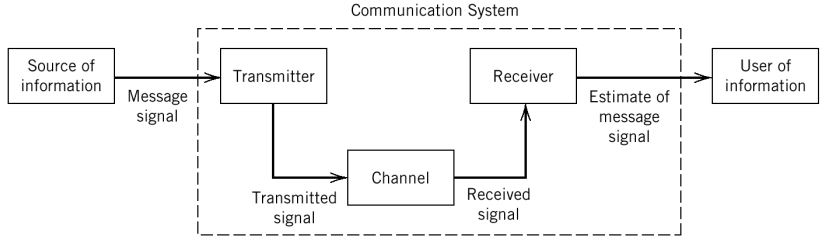
\includegraphics[scale=0.5]{1.JPG}
\end{figure}

%%%%%%%%%%%%%%%%%%%%%%%%%%%%%%%%%%%%%%%%%%%%%%%%%%%%%%%%%%%%%%%%%%%%%%%%%%%%%%%%%%%%%%%%%%%%%%%%%%%%%%%%%%
\subsection{Communication channels}

\begin{itemize}
    \item \textbf{Propagation loss}: Signal strength decay with distance
    \item \textbf{Bandwidth}: Frequency range used for communication 
    \item \textbf{Time variation}: Channel characteristic variation in time 
    \item \textbf{Nonlinearity}: Introduced by some elements e.g. repeaters 
    \item \textbf{Multi-path interference}: Deteriorates signal contents 
\end{itemize}

%%%%%%%%%%%%%%%%%%%%%%%%%%%%%%%%%%%%%%%%%%%%%%%%%%%%%%%%%%%%%%%%%%%%%%%%%%%%%%%%%%%%%%%%%%%%%%%%%%%%%%%%%%
\subsection{Noise}

\begin{itemize}
    \item Unwanted signals in communication system 
    
    \item Two types: 
    \begin{itemize}
        \item \textbf{External noise}: Natural noise, man-made noise
        \item \textbf{Internal noise}: Thermal noise due to channel
    \end{itemize}

    \item Signal-to-noise ratio (SNR): 
    $$
        \text{SNR} = \frac{\text{Signal power}}{\text{Noise power}}
    $$
\end{itemize}

%%%%%%%%%%%%%%%%%%%%%%%%%%%%%%%%%%%%%%%%%%%%%%%%%%%%%%%%%%%%%%%%%%%%%%%%%%%%%%%%%%%%%%%%%%%%%%%%%%%%%%%%%%
\section{Transmitter and Receiver}

\begin{itemize}
    \item \textbf{Transmitter}: Convert source into transmissible format
    \begin{itemize}
        \item \textbf{Modulation}: Carrier-wave parameter based on signal
        \item \textbf{Up-conversion}: Modulated $f(x)$ convert to final RF
    \end{itemize}

    \item \textbf{Receiver}: Reconstruct original signal from modulated 
    \begin{itemize}
        \item \textbf{Down-conversion}: Convert to original RF
        \item \textbf{Demodulation}: Convert to original signal 
    \end{itemize}

    \item Some degradation depending on channel and modulation
\end{itemize}

\pagebreak
%%%%%%%%%%%%%%%%%%%%%%%%%%%%%%%%%%%%%%%%%%%%%%%%%%%%%%%%%%%%%%%%%%%%%%%%%%%%%%%%%%%%%%%%%%%%%%%%%%%%%%%%%%
\section{Objectives of system design}

\begin{itemize}
    \item Primary resources in communication design:
    \begin{itemize}
        \item Transmitted power 
        \item Channel bandwidth 
    \end{itemize}

    \item Deliver message efficiently and reliably within constraints
    \begin{itemize}
        \item Efficiency: Number of transmitted bits in unit power 
        \item Reliability: SNR or Error Probability
    \end{itemize}
\end{itemize}

%%%%%%%%%%%%%%%%%%%%%%%%%%%%%%%%%%%%%%%%%%%%%%%%%%%%%%%%%%%%%%%%%%%%%%%%%%%%%%%%%%%%%%%%%%%%%%%%%%%%%%%%%%
\subsection{Shannon capacity formula}

\begin{itemize}
    \item Maximum rate of reliable transmission: 
    $$
        C = W\log(1+\text{SNR})
    $$
    where $W$ (Hz) is the bandwidth of a channel 

    \item Almost $0$ error probability if signal rate less than C 
\end{itemize}




%%%%%%%%%%%%%%%%%%%%%%%%%%%%%%%%%%%%%%%%%%%%%%%%%%%%%%%%%%%%%%%%%%%%%%%%%%%%%%%%%%%%%%%%%%%%%%%%%%%%%%%%%%
\end{document}
